\chapter{High performance computing and the LBM}\label{sec:hpc}
To benefit as much as possible from a numerical method, it is crucial
that it is implemented in an efficient manner. In this chapter, some
important aspects of this is discussed. In order to write a code that
allows for efficient execution, some principles behind how a computer
operates must be considered in detail. This varies considerable
between various computer architectures. In this chapter, the
discussion is limited to computers that implement the x86(-64)
architecture which is a very common alternative among today's
workstations.

\section{The pipeline}
To execute an instruction, several parts of the hardware is typically
involved. The basic idea of pipelining is to allow these different
parts of hardware to operate simultaneously. For example at the same
time as an instruction is executed the instruction that will be
executed in the next clock cycle may be decoded. In principle all
modern computer architectures are pipelined.

The x86 architecture is a CISC (Complex instruction set computing)
arcitecture which means that it consists of a rather large number of
specific instructions. The opposite case is a RISC (Reduced
instruction set computing) architecture that only has a very few but
general instructions. Due to the pipelining, an important property of
RISC is that the instructions execute in one clock cycle great
performance benefit of the RISC architectures. The modern CISC
architectures is however said to be RISC-like and has also the ability
of pipelining. Since The CISC pipelining is rather complicated,
e.g. the Intel Xeon processor in the computer that this text is
written on has a 20 stage pipeline \cite{intel-xeon}. The principle is
however the same as in the RISC case, therefore a brief explanation of
the classical RISC pipeline is given here. The RISC pipeline consists
of the following 5 stages:

\begin{enumerate}
  \item Fetch of instruction 
  \item Decoding of fetched instruction
  \item Execution of instruction
  \item Memory access
  \item Write result to register
\end{enumerate}

Each of these tasks takes one clock cycle to perform. Thus if a single
instruction, e.g. an addition is to be computed, it will take 5 clock
cycles. This is the start-up time of the pipeline and when it is
filled, one instruction per clock cycle is executed. 

In order to achieve as many instructions computed per time as
possible, the objective must be to keep the pipeline filled. However,
situations may arise when this seems difficult. For instance when
there are dependencies between stages, e.g. that the output from
execution E1 is the input to execution E2. This means that E2 may have
to wait for E1 to finish and the pipeline is stalled for a number of
clock cycles. An other situation is the following:

\begin{verbatim}
...
if(a == 3)
  a = 2 
else
  a++
end if
...
\end{verbatim}
Here as the instruction for the if statement has been fetched, it is
not clear what instruction will be fetched in the next clock
cycle. The if statement must first be evaluated before such a decision
can be made. Thus the pipeline is stalled also in this case. From this
example we conclude that having branch statements in places where they
are often executed, e.g. in loops, is a performance loss and should be
avoided. Sometimes it is not avoidable and therefore, modern compilers
have a way of dealing with this issue. A usual approach is to guess
which branch that will be taken and continue to fill the pipeline with
its content. Some compilers always ``guess'' the branch following the
first conditional statement, in this case it is important for the
programmer to know this in order to put the most likely case
here. \cite{wiki-pipeline}

The conclusion from this section is that unnecessary branches and data
dependency in loops must be avoided and when this may not be the case,
one must make sure that the compiler does its best to optimise these
situations. 


\nomenclature{CISC}{Complex Instruction Set Computing}
\nomenclature{RISC}{Reduced Instruction Set Computing}
\nomenclature{CPU}{Central Processing Unit}
\nomenclature{PU}{Processing Unit}


\section{Locality}
In a modern computer, memory is arranged in a subsequent manner,
different types of memory are used in order to keep cost down and
speed up. Closer to the CPU small and fast memory types are used those
are often referred to as cache memories and are an intermediate memory
level between the CPU registers and the RAM. In today's computers,
usually several layers of cache memories are used. A schematic image
of this is shown in fig. \ref{fig:hpc:mem}.

\begin{figure}
\begin{center}
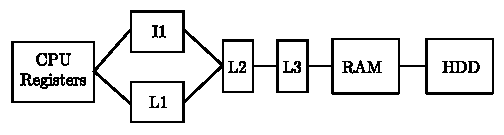
\includegraphics[width=0.6\textwidth]{fig/mem.pdf}
\end{center}
\caption{Sketch of memory layout in a modern computer. I1 is the
  instruction cache and L1 the smallest data cache. Memories to the
  left are faster and smaller but more expensive. }
\label{fig:hpc:mem}
\end{figure}

When data are to be fetched from the memory into the registers of the
CPU, it is first looked for in the L1 data cache if it is not present
there, the next level cache (L2) are tried and so on. If the data is
not present in any level of the cache it has to be read from the main
memory, this is often referred to as a cache miss and is the opposite
to a cache hit. To fetch data from the main memory takes, for a modern
CPU, the same amount of time in which the CPU may execute about 100
instructions \cite{wiki-mem}. It is in other words much slower than to
fetch from the cache.

As a cache miss occurs, not only the value at the specific address
that was wanted but also data that is adjacent to that value is
fetched and placed in the cache. This collection of data is called a
cache line. In order to keep down memory latency, it may be a good
idea if the other data in the cache line could be used before it is
overwritten. This is the concept of locality, to keep data adjacent in
memory that are to be used adjacent in time. It is a major topic in
high performance computing and great performance losses may arise if
the principle of locality is not considered.

%\todo{example}

\subsection{Locality and the LBM}
In an implementation of the lattice-Boltzmann method, the main
quantity that is used in computation is the distribution
function $\fii$. It is in the implementation realised as an array of
dimension $\nx \times \ny \times Q$ where $Q$ is the number of
directions in the discretised velocity space. Basically, two models
for arranging $\fii$ in memory exist:

\begin{description}
  \item[A.] All directions for a certain node are placed adjacent in
    memory.
  \item[B.] All nodes for a certain direction are placed adjacent in
    memory.
\end{description}

To decide which model that is chosen, they must be examined with
respect to locality and the algorithm used. The algorithm in the LBM
consists of two main parts, i.e. the collision step and the streaming
step. In a BGK collision, to update $\fii$, i.e. the distribution
function for direction $i$, the distribution functions for all other
directions from this node must be used in order to compute the
equilibrium distribution. Thus for the collision step, model A would
give better locality. On the other hand, in the streaming step, to
stream $\fii$, the streaming must start at the nodes where, $i$ is
directed out of the domain. Otherwise will unstreamed distributions be
overwritten. Thus it is not directly possible to stream all directions
for a certain node adjacent in time but instead all nodes for a
certain direction. This suggests that model B is more favourable for
the streaming step. There is an approach proposed in \cite{mikael}
where two arrays are used for $\fii$ and in the streaming step, the
streaming is done from one array to the other and nothing is
overwritten. This requires however twice as much memory and it has not
been tested in the implementation done in this work.

$Q$ is typically much smaller than the number of nodes $\nx \times
\ny$. This gives that when a cache line is fetched for model A, same
directions from neighbouring nodes will also be fetched into the cache
and a cache miss will not occur for each node update in the
streaming. In model B, different directions will typically not be
fetched for the same node and in the collision step, a cache miss will
probably occur for each direction. The conclusion is that model A is
better with respect to locality for the ``worst'' part of the
algorithm and is therefore chosen. Tests performed on a laptop with
an Intel Core 2 Duo processor also shows that model A in general gives
better locality.


\nomenclature{L1, L2, L3}{Level 1,2,3 (cache)}
\nomenclature{RAM}{Random Access Memory}
\nomenclature{HDD}{Hard Disk Drive}


\section{Parallelisation}

Parallel computing has, during the last decade, become a major topic
not only in high-performance computing but in other fields of
computing as well. As it gets tougher and tougher to squeeze in more
circuits in a CPU, the idea of having several CPUs (or CPU cores) is
today not only utilised in super computers but in most modern user
workstations as well.

There are mainly two different hardware setups that has to be
distinguished between in parallel computing. Either the memory is
shared between all or distributed locally at each processing unit
(PU). The former is often referred to as shared memory and the latter
to a distributed memory computer. An example of a shared memory
computer would be a workstation having two CPU cores sharing the same
RAM. A system using distributed memory could for instance be a super
computing cluster where several computers (nodes) are connected in a
network.

Obvious differences arise in how the processing units may access data
and communicate data between each other.  In the case with shared
memory computers, common address spaces may be used for communication
and for distributed, messages are passed over the network. As a
programmer there is a major difference in how this is done. Since this
is a common task, there exist software for simplifying the
parallelistation of a code. In distributed computing an interface is
defined for how the communication over the network may be done, this
interface is called MPI (Message Passing Interface). There are several
implementations of MPI, one example is Open MPI \cite{openmpi}. For
shared memory computers OpenMP \cite{openmp} is an API that allows for
a rather effortless way of parallelising a code.

An algorithm may in a varying degree be suited for parallelising. If
there is a lot of data dependence or dependencies in general. It may
be difficult to divide the computation in independent tasks on
different PUs. In the case with the algorithm in lattice-Boltzmann,
the algorithm is very well suited for parallelisation. This is often
considered a great strength of the lattice-Boltzmann method. The
main part of the computation is done in the collision step, and a
collision on a node is computed independently of data from other
nodes. In parallelisation of the streaming step however, communication
between nodes are needed. The win in performing the streaming step in
parallel is much smaller than for the collision step. By this reason
and the fact that a shared memory parallelisation using OpenMP is
chosen, only the collision step is parallelised in this work.

The parallelisation was tested for a sample system of $100 \times 100$
nodes with periodic boundary conditions and large number of time
steps. The speedup was measured for different number of parallel
processes used. The result using 2, 5 and 10 respectively cores is
shown in fig. \ref{fig:hpc:para}. The computer used had more than 10
CPU cores. 

\begin{figure}
\begin{center}
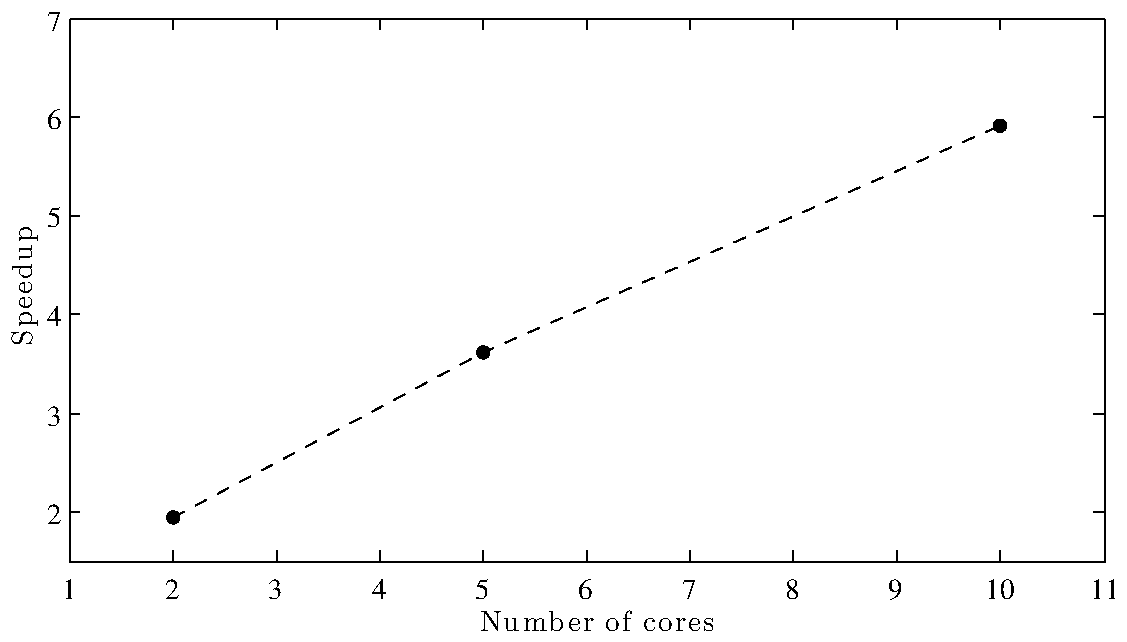
\includegraphics[width=0.9\textwidth]{fig/para.pdf}
\end{center}
\caption[Speedup of the parallelised lattice-Boltzmann code.]{Speedup
    of the parallelised lattice-Boltzmann code. Only the collision
    step with a BGK collision operator and not the streaming step is
    parallelised. The computation was done on a computer with two 12
    cores \texttt{Intel(R) Xeon(R) X5650} CPUs.}
\label{fig:hpc:para}
\end{figure}


\nomenclature{API}{Application Programming Interface}
\nomenclature{MPI}{Message Passing Interface}


\section{LBM implementation}

C++

%\section{Maybe something about profiling}
%men kanske inte tillför något vettigt.

%\section{Choice of programming language}

%\section{Some stats on the performance of the code...}
%Lattice updates/s
